\newpage
\section{529. 扫雷游戏}
\label{leetcode:529}

\subsection{题目}

让我们一起来玩扫雷游戏!

给定一个代表游戏板的二维字符矩阵。'M' 代表一个未挖出的地雷,
'E' 代表一个未挖出的空方块,'B' 代表没有相邻(上,下,左,右,和所有4个对角线)
地雷的已挖出的空白方块,数字('1' 到 '8')表示有多少地雷与这块已挖出的方块相邻,
'X' 则表示一个\textbf{已挖出的}地雷。

现在给出在所有\textbf{未挖出的}方块中('M'或者'E')的下一个点击位置(行和列索引),
根据以下规则,返回相应位置被点击后对应的面板:

\begin{itemize}
  \item 如果一个地雷('M')被挖出,游戏就结束了- 把它改为 'X'。
  \item 如果一个\textbf{没有相邻地雷}的空方块('E')被挖出,修改它为('B'),
    并且所有和其相邻的方块都应该被递归地揭露。
  \item 如果一个至少与一个地雷相邻的空方块('E')被挖出,
    修改它为数字('1'到'8'),表示相邻地雷的数量。
  \item 如果在此次点击中,若无更多方块可被揭露,则返回面板。
\end{itemize}

\textbf{示例 1}:

\begin{verbatim}
  输入: 

  [['E', 'E', 'E', 'E', 'E'],
  ['E', 'E', 'M', 'E', 'E'],
  ['E', 'E', 'E', 'E', 'E'],
  ['E', 'E', 'E', 'E', 'E']]

  Click : [3,0]

  输出: 

  [['B', '1', 'E', '1', 'B'],
  ['B', '1', 'M', '1', 'B'],
  ['B', '1', '1', '1', 'B'],
  ['B', 'B', 'B', 'B', 'B']]
\end{verbatim}

解释:

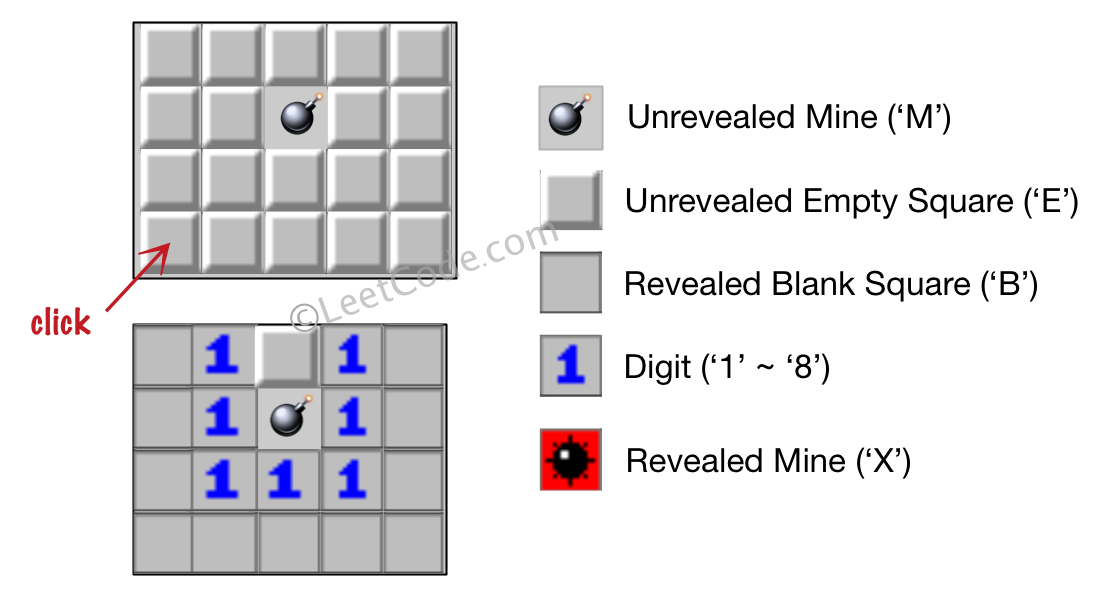
\includegraphics[width=150mm,height=100mm]{images/leetcode/minesweeper_example_1.png}

\textbf{示例 2}:

\begin{verbatim}
  输入: 

  [['B', '1', 'E', '1', 'B'],
  ['B', '1', 'M', '1', 'B'],
  ['B', '1', '1', '1', 'B'],
  ['B', 'B', 'B', 'B', 'B']]

  Click : [1,2]

  输出: 

  [['B', '1', 'E', '1', 'B'],
  ['B', '1', 'X', '1', 'B'],
  ['B', '1', '1', '1', 'B'],
  ['B', 'B', 'B', 'B', 'B']]
\end{verbatim}

解释:

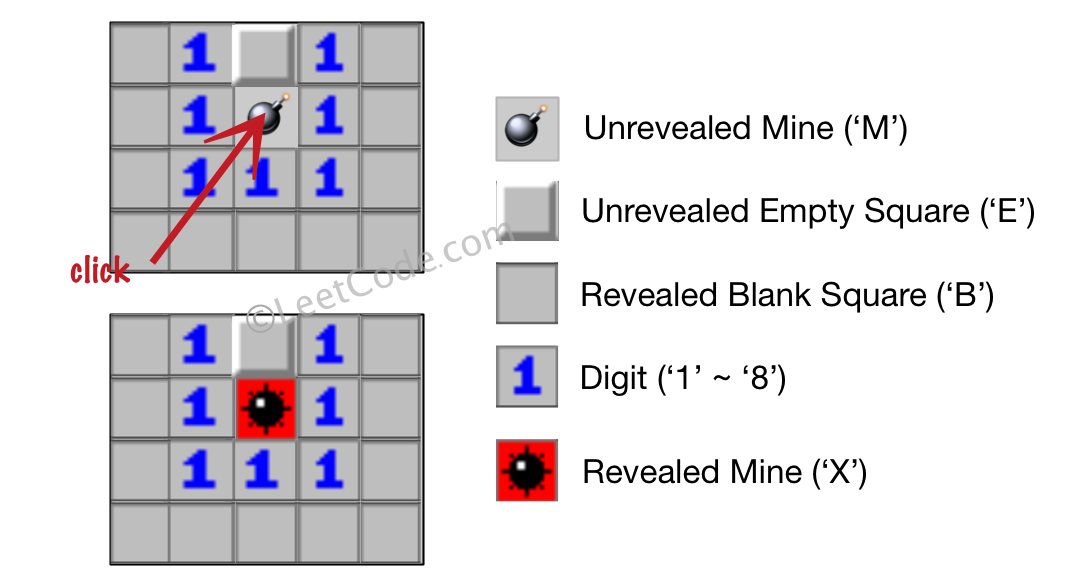
\includegraphics[width=150mm,height=100mm]{images/leetcode/minesweeper_example_2.png}

注意:

\begin{itemize}
  \item 输入矩阵的宽和高的范围为 [1,50]。
  \item 点击的位置只能是未被挖出的方块 ('M' 或者 'E'),
    这也意味着面板至少包含一个可点击的方块。
  \item 输入面板不会是游戏结束的状态(即有地雷已被挖出)。
  \item 简单起见,未提及的规则在这个问题中可被忽略。
    例如,当游戏结束时你不需要挖出所有地雷,考虑所有你可能赢得游戏或标记方块的情况。
\end{itemize}

\subsection{参考题解}

\begin{verbatim}
/**
 * @param {character[][]} board
 * @param {number[]} click
 * @return {character[][]}
 */
var updateBoard = function(board, click) {
  let queue = [];
  queue.push(click);
  while (queue.length > 0) {
    let curClick = queue.shift();
    let curRow = curClick[0];
    let curCol = curClick[1];
    if (board[curRow][curCol] === 'M') {
      board[curRow][curCol] = 'X';
      break;
    } else if (board[curRow][curCol] === 'E') {
      let mineCount = findAdjoinMine(board, curRow, curCol);
      if (mineCount === 0) {
        board[curRow][curCol] = 'B';
        let ms = getAdjoinE(board, curRow, curCol);
        for (let i = 0; i < ms.length; i += 1) {
          queue.push(ms[i]);
        }
      } else {
        board[curRow][curCol] = '' + mineCount;
      }
    }
  }
  return board;
};

const dirs = [
  [-1, 0],
  [1, 0],
  [0, -1],
  [0, 1],
  [-1, -1],
  [1, 1],
  [-1, 1],
  [1, -1],
];

function getAdjoinE(board, row, col) {
  let result = [];
  for (let i = 0; i < dirs.length; i += 1) {
    const newRow = row + dirs[i][0];
    const newCol = col + dirs[i][1];
    if (isValidIndex(board, newRow, newCol)) {
      if (board[newRow][newCol] === 'E') {
        result.push([newRow, newCol]);
      }
    }
  }
  return result;
}

function findAdjoinMine(board, row, col) {
  let count = 0;
  for (let i = 0; i < dirs.length; i += 1) {
    const newRow = row + dirs[i][0];
    const newCol = col + dirs[i][1];
    if (isValidIndex(board, newRow, newCol)) {
      if (board[newRow][newCol] === 'M') {
        count += 1;
      }
    }
  }
  return count;
}

function isValidIndex(board, row, col) {
  if (row < 0 || col < 0) {
    return false;
  }
  if (row >= board.length) {
    return false;
  }
  if (col >= board[0].length) {
    return false;
  }
  return true;
}
\end{verbatim}